\chapter{Basic Underlying Techniques}

To understand how feature location techniques work it is important to understand a few basic techniques that are commonly used to create or improve feature location. All the basic techniques  will be exemplary executed on the previously introduced Freemind-example in chapter~\ref{ch:Freemind Example}.

\section{Formal Concept Analysis (FCA)}
\emph{Formal Concept Analysis} (short: \emph{FCA}) is a predominantly mathematical approach to identify groups of classes and methods compared by the sharing of attributes. Therefor the \emph{FCA} regards the binary relation between all objects and attributes and therefor can also provide a model to analyze hierarchy, because hierarchy structures often have similar relations. 
\begin{wrapfigure}[16]{r}{0.45\textwidth}
  \fbox{
  \begin{tikzpicture}
   % nodes
   \node[block] (a) {$\sigma_1$ = MindMapMapModel.doAutomaticSave.run()};
   \node[block] (b)  [below of=a, node distance = 2 cm] {\color{gray}Mind \color{red}Map \color{blue}Model \color{yellow}do \color{green}Automatic \color{purple}Save \color{orange}run};
   \node[block] (c)  [below of=b, node distance = 2 cm] {\color{gray}mind \color{red}map \color{blue}model \color{yellow}do \color{green}automatic \color{purple}save \color{orange}run};
   \node[block] (d)  [below of=c, node distance = 3.5 cm] {
  \begin{center}
    \begin{tabular}{| l | c |}
      \hline
      & $\sigma_1$ \\ \hline
      \color{gray}mind & \checkmark \\ \hline
      \color{red}map & \checkmark \\ \hline
      \color{blue}model & \checkmark \\ \hline
      \color{yellow}do & \checkmark \\ \hline
      \color{green}automatic & \checkmark \\ \hline
      \color{purple}save & \checkmark \\ \hline
      \color{orange}run & \checkmark \\ \hline
      \color{black} other &  \\ \hline
    \end{tabular}
  \end{center}
};

   % edges
   \draw[->] (a) -- node[right] {1. declare every $w_i$} (b);
   \draw[->] (b) -- node[right] {2. decapitalize the $w_i$'s} (c);
   \draw[->] (c) -- node[right] {3. create table} (d);
  \end{tikzpicture}}
  \caption{\#1 of the Freemind Example as example}
  \label{flowchart}
\end{wrapfigure}


The \emph{FCA}'s goal is to define so called \emph{concepts}. A \emph{concept} is a tuple of extension, the objects that belong to a concept, and intension, all the attributes that \underline{every} object of the extension has.
In order to be able to derive such a \emph{concept} the \emph{FCA} creates an incidence table. The table can be derived in 3 steps as seen in Fig. ~\ref{flowchart}:
\begin{enumerate}
  \item declaring every word in the objects and methods as $w_i$ to a new $i$ if the word isn't already defined
  \item decapitalizing every $w_i$
  \item creating the table with every decapitalize word as a row and every $\sigma$ as a column. The cells $c_ij$ are checked if  $\sigma$ contains the word $w_i$
\end{enumerate}
\pagebreak
\begin{wrapfigure}[20]{l}{0.6\textwidth}
    \centering
    \begin{tabular}{| l | c | c | c | c | c | c | c | c |}
      \multicolumn{1}{c}{objects} & \multicolumn{1}{c}{$\sigma_1$} & \multicolumn{1}{c}{$\sigma_2$} & \multicolumn{1}{c}{$\sigma_3$} & \multicolumn{1}{c}{$\sigma_4$} & \multicolumn{1}{c}{$\sigma_5$} & \multicolumn{1}{c}{$\sigma_6$} & \multicolumn{1}{c}{$\sigma_7$} & \multicolumn{1}{c}{$\sigma_8$} \\ 
      \multicolumn{1}{c}{$\downarrow$} &  \multicolumn{1}{c}{$\downarrow$} & \multicolumn{1}{c}{$\downarrow$} & \multicolumn{1}{c}{$\downarrow$} & \multicolumn{1}{c}{$\downarrow$} & \multicolumn{1}{c}{$\downarrow$} & \multicolumn{1}{c}{$\downarrow$} & \multicolumn{1}{c}{$\downarrow$} & \multicolumn{1}{c}{$\downarrow$} \\ \hline
      action       	&			  	&                    &                     &                    &                    &                     &                    & \checkmark \\ \hline 
      automatic 	& \checkmark 	& \checkmark &                     &                    &                    &                     &                    &                    \\ \hline
      controller  	&			  	&                    &                     &                    &                    &                     &                    & \checkmark \\ \hline
      do 			& \checkmark 	& \checkmark &                     &                    &                    &                     &                    &                    \\ \hline
      file 			&			    	&                    &                     &                    &                    &                     &                    &                    \\ \hline
      free 		&			    	&                    &                     &                    & \checkmark & \checkmark  &                    &                    \\ \hline
      internal 	&			    	&                    & \checkmark	 &                    &                    &                     &                    &                     \\ \hline
      map 		& \checkmark	& \checkmark & \checkmark  & \checkmark &                    &                     & \checkmark & \checkmark \\ \hline
      mind 		& \checkmark	& \checkmark & \checkmark  & \checkmark & \checkmark & \checkmark  & \checkmark & \checkmark \\ \hline
      model 		& \checkmark	& \checkmark & \checkmark  & \checkmark & \checkmark & \checkmark  & \checkmark & \checkmark \\ \hline
      node 		&			    	&                    &                     &                    &                    & \checkmark  & \checkmark &                     \\ \hline
      performed 	&			    	&                    &                     &                    &                    &                     &                    & \checkmark  \\ \hline
      run 			& \checkmark 	&                    &                     &                    &                    &                     &                    &                     \\ \hline
      save 		& \checkmark	& \checkmark & \checkmark  &			     & \checkmark & \checkmark  & \checkmark &				 \\ \hline
    \end{tabular}
     \caption{The complete incidence table of the Freemind Example}
     \label{FCA_finaltable}
\end{wrapfigure}

Keeping the methods numbers  as we did we get Figure 3.2 as a result. Mathematically it leads us to defining $O$ as a set of objects, $A$ as a set of attributes and $R$ as the set of relations $r = (o,a) \quad o\in O,a\in A$ as derivable of the table. Also we define that \newline
$\sigma(O) = \{a \in A | (o,a) \in R, \forall o \in O \}$  \quad "all attributes that every $o\in O$ has" \newline
 $\rho(A)= \{o\in O|(o,a)\in R, \forall a\in A \}$  \quad "all objects that every $a\in A$ has" \newline
So a concept can be declared as a tuple $c=(O,A)$ so that $A=\rho(0)$ and $O=\sigma(A)$. So $O$ is the extension and $A$ is the intension.

From there it is very easy to see, that the set of all concepts $C$ is a partial order (\emph{superconcept} - \emph{subconcept}) defined as: \newline
\begin{center}
  \vspace{-2em}
  \begin{tabular}{ r c l }
  $ (O_1,A_1) \le (O_2, A_2)$ & $\Leftrightarrow$ & $O_1 \subset O_2 \ or \ A_1 \subset A_2$. \\
  \end{tabular}
\end{center}
\vspace{-1em}
Which leads to the definition that $C, \le$ form a concept lattice and in our example it's a taxonomy of name tokens.

%END FCA%

%BEGINN LATENT SEMANTIC%
\section{Latent Semantic Indexing (LSI)}
\label{ch:lsi}
\begin{wrapfigure}[17]{l}{0.5\textwidth}
  \centering
    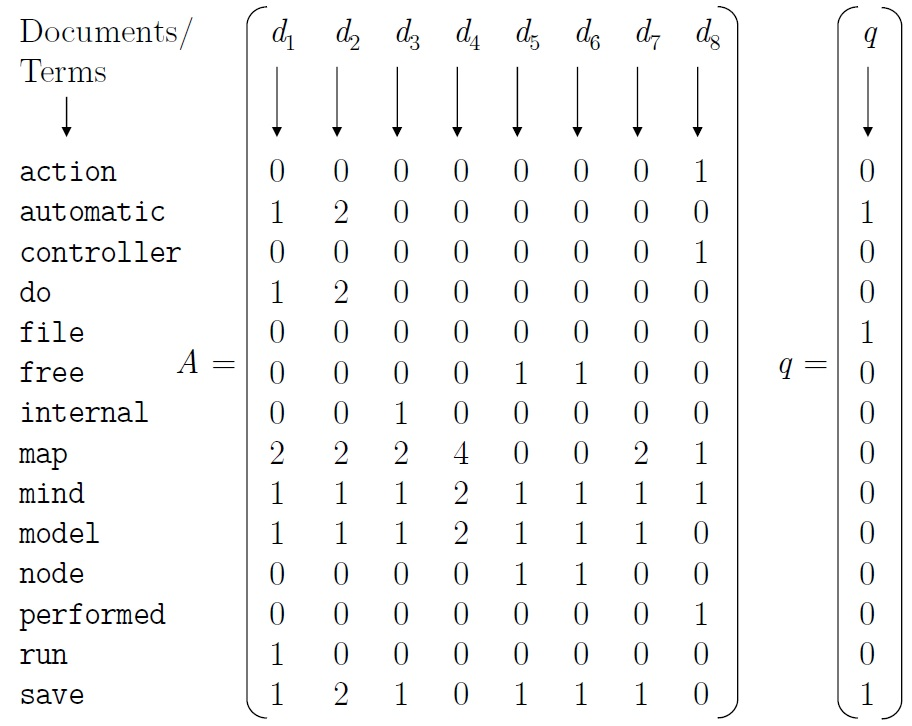
\includegraphics[width=\linewidth]{src/pic/term_document_matrix}
    \label{term-document-matrix}
  \caption{The term-document matrix}
\end{wrapfigure}
The \emph{Latent Semantic Indexing}(short: \emph{LSI}) is an automatic statistical technique. It derives to a given document a vector representation of the query and the corpus by creating a term-document matrix of co-occurring terms. A term $t_i$ is a word, as a tokenized and decapitalized word of the methods ordered alphabetically and is represented in a row of the matrix. A document $d_j$, which are in our example the different method- and class names, are represented as the columns of the matrix. So the matrix, shown in Fig.~\ref{term-document-matrix}, looks very similar to the table of FCA (Fig.~\ref{FCA_finaltable}) with the difference of an unsigned integer value $v_ij$, representing how often a document $d_j=MindMapMapModel.doAutomaticSave.run()$ contains token $t_i$, i.e. $d_1$ contains the token $t_7=map$ twice, but the token $t_2=automatic$ only once and doesn't contain $t_1=action$ at all. Also a query \emph{q} is given, which has a \emph{1} at the terms \emph{automatic}, \emph{save} and \emph{file} representing the feature that should be analyzed. 


\begin{wrapfigure}[15]{l}{0.5\textwidth}
  \centering
  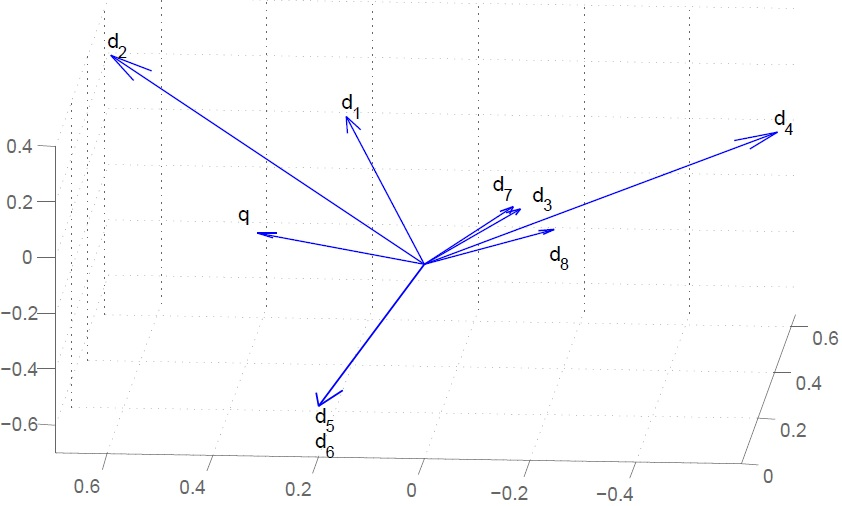
\includegraphics[width=\linewidth]{src/pic/lsf-vectors}
  \label{lsf_vectors}
  \caption{The vector representation of the documents $d_j$ and the query $q$ from the Freemind Example~\ref{ch:Freemind Example}}
\end{wrapfigure}
By normalizing and decomposing using a singular value decomposition the documents can be put into vector representation so that every document has a vector representing their equality to the query $q$. Taking the $cosine()$ of the query $q$ and a document $d_j$ it is possible to measure the similarity. If a document and a query are equal the spreading angle would be $0$ and therefor the best possible similarity is given by $cosine(0)=1$. Also the worst possible angle is $180$, which is equal to document "pointing in the opposite direction", and therefor the worst similarity is given by $cosine(180)=-1$. The common interpretation of the values, regarding that $D$ is the set of all documents, is, that the set $\{d_i \in D| cosine(d_i,q) \ge 0 \} \subseteq D$ are considered to be a related to the query of interest, hence every other document is not. It's simple to see that a document is more similar if it points in the same general direction as the query, because of the shared terms. In the Freemind Example the document $d_2=\color{red}MindMapMapModel\color{black}.\color{red}do\color{green}AutomaticSave\color{black}.\color{red}do\color{green}AutomaticSave\color{black}$ is the most similar to the query $q=\color{green}automaticSaveFile\color{black}$, while $d_8=\color{red}MindMapController\color{black}.\color{red}actionPerformed\color{black}$ is the least similar.
\begin{center}
  \begin{tabular}{ c c c c c c c c }
    \hline
    $d_1$ & $d_2$ & $d_3$ & $d_4$ & $d_5$ & $d_6$ & $d_7$ & $d_8$ \\ \hline
    0.6319 & 0.8897 & -0.2034 & -0.5491 & 0.2099 & 0.2099 & -0.1739 & -0.6852 \\ \hline
  \end{tabular}
\end{center}
Like previously mentioned $d_2$ is the most similar to $q$, because of the "pointing in the same general direction", which it now proven by having the highest value $cosine(d_2,q)=0.8897=max \{ cosine(d_i,q) | d_i \in D \} $ and also $d_8$ is the least similar with a value $cosine(d_8,q)=-0.6852=min\{cosine(d_i,q) | d_i \in D\}$.
  

%END LATENT SEMANTIC
\section{Term Frequency - Inverse Document Frequency (tf-idf)}
%BEGINN TERM FREQUENCY
The \emph{term frequency - inverse document frequency} technique is a statistical technique to derive a feature to a given intension. It measures the importance of a term or multiple terms to documents by its frequency of appearing. The terms are terms of the intension of the feature that is wanted to be analyzed. In a simple way it can be described as: "the more frequent a term occurs in the document, the more relevant the document is to the term". \newline
This is mathematically described as the $document frequency tf=(t,d)$, counting how often the term $t$ is contained in the document $d$.
In our example the term $t_2 = save$ appears in $d_3$ once and the term $t_1 = automatic$ doesn't appear at all so: $tf(t_2,d_3) = 1$ and $tf(t_1,d_3)=0$. \newline
Doing that for the terms $t_1 = automatic, t_2 = save$ and $t_3 = file$ and the documents $d_1$ to $d_8$ we get the matrix shown in Fig.~\ref{term-document-matrix}.
The main problem of this technique is, that uninformative terms appearing within a document-set, often referred as \emph{corpus} and shortened by $D$, maybe even multiple times can distract from terms, which are mentioned less frequent but are more relevant. To compensate that, the technique relativizes by calculating how many documents contain the term and normalizing it. If it's a commonly used term shared by many documents this term can't be taken as a measurement to differentiate between documents. Or colloquially "the more documents include a term, the less this term discriminates between documents". \newline
So the so-called \emph{inverse document frequency (idf(t))} is calculated as
\begin{center} $idf(t) = log((|D|)/|\{ d \in D | t \in d \}|)$  \end{center}
with $D$ still being the set of documents. And the final \emph{term frequency - inverse document frequency} is the multiplication of both scores, so:
\begin{center} \emph{tf-idf}$(t,d) = tf(t,d) * idf(t)$\end{center}
Regarding our example we can compute the $idf$ of our terms:

%\begin{itemize}
%  \item $t_1 = automatic : idf(t_1) = log(8/2)$ 
%  \item $t_2 = save : idf(t_2)=log(8/6)$
%  \item $t_3 = file : idf(t_3)=0$ 
%\end{itemize}

\begin{table}[h]
  \centering
  \begin{tabular}{l}
    $t_1 = automatic : idf(t_1) = log(8/2)$  \\
    $t_2 = save : idf(t_2)=log(8/6)$ \\
    $t_3 = file : idf(t_3)=0$ 
 \end{tabular}
\end{table}

Like in the example if the focus isn't on one term but on a set of terms the \emph{tf-idf(t,d)} values to a document $d$ are added up. So finally the matrix can be derived as it is shown in Table \ref{tab:tfidf_table}.

\begin{table}[h]
  \centering
  \begin{tabular}{| l | c | c | c | c | c | c | c | c |}
    \hline
    & $d_1$ & $d_2$ & $d_3$ & $d_4$ & $d_5$ & $d_6$ & $d_7$ & $d_8$ \\ \hline
    $t_1 = automatic$ & 0.6021 & 1.2041 & 0 & 0 & 0 & 0 & 0 & 0 \\ \hline
    $t_2 = save$ & 0.1249 & 0.2499 & 0.1249 &0 & 0.1249 & 0.1249 & 0.1249 & 0 \\ \hline
    $t_3 = file $ & 0 & 0 & 0 & 0 & 0 & 0 & 0 & 0 \\ \hline \hline
    $\sum\nolimits_{i=1}^3$\emph{tf-idf}$(t_i,d_j)$ & 0.727 & 1.454 & 0.1249 & 0 & 0.1249 & 0.1249 & 0.1249 & 0\\ \hline
  \end{tabular}
  \label{tab:tfidf_table}
  \caption{Term Frequency - Inverse Document Frequency}
\end{table}

%END TERM FREQUENCY
\section{Hyper Link Induced Topic Search (HITS)}
%BEGIN HITS

The \emph{Hyper Link Induced Topic Search} (short: \emph{HITS}) is a page ranking algorithm for web mining\footnote{\label{foot:1}web mining is the analysis step of the knowledge discovery in databases process within the World Wide Web CITE}, which is the counterpart of the famous \emph{Google Page Rank}-algorithm and is currently used by the \emph{Ask Search Engine} \cite{wiki:HITS}. Its basically used to get websites that correspond best to a given input, like every search engine. 
The \emph{HITS}-algorithm distinguishes between two forms of web pages, which aren't necessarily disjoint:
\begin{enumerate}
  \item hub \newline
  A hub is a web page pointing towards other web pages , which can be a hub, an authority or even both. A pragmatism is to say: "a good hub points to many authorities."
  \item authority \newline
  An authority is a web page, that other pages point to in order to cite or prove. The rule of thumb is: "a good authority is pointed by many good hubs."
\end{enumerate}

Regarding the definition of hubs and authorities it seems quite natural to define a directed graph $G=(V,E)$ with vertices $V$ = web pages and edges $E = \{(v,w) | v \textrm{ refers to }w\}$ (also called \emph{links}) .
A hubscore is the number of authorities the hub refers to. An authorityscore is a number of good links that refer towards this authority. Both are initialized with 1.
Keeping the graph $G$ in mind the hub- and authority scores can be defined as the following. \newline
\begin{center}
  \begin{tabular}{ r c l }
    authority score of page $p$ & & $A_p=\{ \sum\nolimits_{\{ q | (q,p) \in E \} } H_q \}$ \\
    hub score of page $p$ & & $H_p = \{ \sum\nolimits_{\{ q | (p,q) \in E \} } A_q \}$ \\
  \end{tabular}
\end{center}
Given the two values the graph can be rewritten as $G'=(V',E')$ with $V'=\{ (p, H_p, A_p)| \forall p\in V\}$ and $E' = E$.
By iterating over the graph the values of $H_p$ and $A_p$ are calculated for every page $p$.  In order to don't just count up to infinity the values have to be normalized like the following:
\begin{center}
  \begin{tabular}{ r c l }
    normalizing the authority score of page $p$ & & $A_p= A_p/\sqrt{\sum\nolimits_{ (q,H_q,A_q) \in V' } A_q^2}$ \\
    normalizing the hub score of page $p$ & & $H_p = H_p/\sqrt{\sum\nolimits_{\{(q,H_q,A_q) \} \in V'} H_q^2}$ \\
  \end{tabular}
\end{center}
The normalized values satisfy the condition, that $\sum\nolimits_{\{(p,H_p,A_p) \} \in V'} H_p^2 = \sum\nolimits_{\{(p,H_p,A_p) \} \in V'} A_p^2 = 1$.

\begin{wrapfigure}[17]{l}{0.6\textwidth}
  \centering
  \begin{tikzpicture}
  \tikzset{vertex/.style = {shape=ellipse,draw,minimum size=1.5em}}
  \tikzset{edge/.style = {->,> = latex'}}
  % vertices
  \node[vertex] (p1) at  (1,4) {($p_1$, 1, 0)};
  \node[vertex] (p2) at  (5,2) {($p_2$, 0, 1)};
  \node[vertex] (p3) at  (1,2) {($p_3$, 1, 2)};
  \node[vertex] (p4) at  (5,0) {($p_4$, 1, 2)};
  \node[vertex] (p5) at (-1,0)  {($p_5$, 1, 1)};
  \node[vertex] (p6) at (-1,-2) {($p_6$, 0, 1)};
  \node[vertex] (p7) at (2,0)  {($p_7$, 2, 1)};
  \node[vertex] (p8) at (2,-2) {($p_8$, 2, 0)};
  %edges
  \draw[edge] (p1)  to (p3);
  \draw[edge] (p4)  to (p2);
  \draw[edge] (p7)  to (p3);
  \draw[edge] (p3)  to (p5);
  \draw[edge] (p5)  to (p6);
  \draw[edge] (p7)  to (p4);
  \draw[edge] (p8)  to (p4);
  \draw[edge] (p8)  to (p7);
  \end{tikzpicture}
  \caption{The graph G}
  \label{hits_graph_g}
\end{wrapfigure}

Applying the \emph{HITS}-algorithm to program code hubs can be colloquially described as methods, that call many other methods, and authority's can be described as methods, that implement a function.\newline
In the Freemind Example the first graph will look very similar to the class diagram, as it is shown in Fig ~\ref{hits_graph_g}. The class \#i will refer to page $p_i$.
After transferring it into the graph of the form of $G'$ and after the first iteration the graph looks like Fig.~\ref{hits_graph_g}. \newline
Including the normalization the graph $G'$ looks like Fig.~\ref{hits_graph_after_first_iteration}. The normalization was done by calculating for every $H_p$ and $A_p$ of a page $p$ as:\newline
\begin{center}
  \begin{tabular}{ r c l }
    $H_p$ & = &$H_p / \sqrt{1^2+0^2+1^2+1^2+1^2+2^2+0^2+2^2} = H_p/ \sqrt{12}$ and \\
  $A_p$ & = &$ A_p / \sqrt{0^2+1^2+2^2+2^2+1^2+1^2+1^2+0^2} = A_p/ \sqrt{12}$. \\
  \end{tabular}
\end{center}  
  
\begin{figure}
  \centering
  \begin{tikzpicture}
  \tikzset{vertex/.style = {shape=ellipse,draw,minimum size=1em}}
  \tikzset{edge/.style = {->,> = latex'}}
  % vertices
  \node[vertex] (p1) at  (1,4) {($p_1$, $\frac{1}{\sqrt12}$, 0)};
  \node[vertex] (p2) at  (8,2) {($p_2$, 0, $\frac{1}{\sqrt12}$)};
  \node[vertex] (p3) at  (1,2) {($p_3$, $\frac{1}{\sqrt12}$, $\frac{2}{\sqrt12}$)};
  \node[vertex] (p4) at  (8,0) {($p_4$, $\frac{1}{\sqrt12}$, $\frac{2}{\sqrt12}$)};
  \node[vertex] (p5) at  (-2,0) {($p_5$, $\frac{1}{\sqrt12}$, $\frac{1}{\sqrt12}$)};
  \node[vertex] (p6) at  (-2,-2) {($p_6$, 0, $\frac{1}{\sqrt12}$)};
  \node[vertex] (p7) at  (3,0) {($p_7$, $\frac{2}{\sqrt12}$, $\frac{1}{\sqrt12}$)};
  \node[vertex] (p8) at  (3,-2) {($p_8$, $\frac{2}{\sqrt12}$, 0)};
  %edges
  \draw[edge] (p1)  to (p3);
  \draw[edge] (p4)  to (p2);
  \draw[edge] (p7)  to (p3);
  \draw[edge] (p3)  to (p5);
  \draw[edge] (p5)  to (p6);
  \draw[edge] (p7)  to (p4);
  \draw[edge] (p8)  to (p4);
  \draw[edge] (p8)  to (p7);
  \end{tikzpicture}
  \caption{G' after the first iteration with normalizing the scores}
  \label{hits_graph_after_first_iteration}
\end{figure}

%END HITS
%\clearpage









































